\section{Authenticated Encryption with Associated Data}
% Questions:
% what is S_r and S_c?
% What is a Nonce And Tag?
After many years of relying on traditional methods for encryption and authentication through 'generic composition,' new constructions have emerged over the past two decades. They achieved both privacy and authenticity simultaneously and often more efficiently than solutions using generic composition.
\newline
In many environments we do not only have to encrypt and authenticate the message or payload, but also wish to include auxiliary data (like the header of a network packet) which should be authenticated, but left unencrypted. \cite[Chapter 1]{Black2005}
% Umschreiben
The reason being that routers must be able to read the headers of packets in order to know how to properly route them. This need spurred some designers of AE schemes to allow “associated data” to be included as input to their schemes. Such schemes have been termed AEAD schemes (Authenticated Encryption with Associated Data) which rely on symmetric key cryptography.\footnote[1]{\textbf{Symmetric key cryptography}, also called secret or single-key cryptography, uses the same key to both encrypt and decrypt information and is used primarily to ensure data confidentiality. In cases where the information is encrypted and decoded by the same person, there is no need to share the secret key. However, when these operations involve different people or equipment, it is necessary that the secret key be previously combined through a secure communication channel. Examples of cryptographic methods that use a symmetric key are: DES, AES, Blowfish, RC4, 3DES, and IDEA. \cite{Alencar2022Cryptography}}
A notion which was first formalized by Rogaway \cite{10.1145/586110.586125}.

% \subsection{What is AEAD}
% % UMSHREIBEN! 
% AEAD is a cryptographic method that combines encryption and authentication in a single operation. It allows for secure encryption of data while also providing integrity protection. AEAD schemes take plaintext data, associated data (which is authenticated but not encrypted), and a secret key as input, and produce ciphertext along with authentication tags as output. The ciphertext ensures confidentiality, while the authentication tags ensure integrity and authenticity of both the ciphertext and associated data. AEAD schemes are commonly used to protect the confidentiality and integrity of data in various applications, including communication protocols, file systems, and storage systems . \cite{Black2005}

\subsection{Ascon AEAD Scheme} % also explain that im talking about each step and whu its done to make it secure or able to work
In this section, we dive into the Ascon-128 scheme, which, along with Ascon-128a, has been designated as the “primary choice” for lightweight authenticated encryption in the final portfolio of the CAESAR competition. These schemes are notable for their robust security, with no known vulnerabilities. The most effective attacks target only the versions with reduced rounds—specifically, the initialization reduced to 7 out of 12 rounds—and these are still far from posing a practical threat. Notably, benchmarks have demonstrated that Ascon excels in efficiency, particularly for short messages, confirming its status as a state-of-the-art lightweight encryption method. \cite[Chapter 1]{Ascon-v1.2}


\subsection{Authenticated Encryption $E_{k,r,a,b}$}
The encryption procedure $E_{k,r,a,b}$ takes the following inputs:
\begin{itemize}
    \item Secret key $K$ with $k$ bits.
    % find Citation! and make footnote!
    \item Nonce (public message number) $N$ with 128 bits. \footnote[2]{The term "\textbf{nonce}" stands for "number used once," a unique value that must be used only once with a given key for a particular encryption operation to ensure that each operation generates a unique ciphertext, even if the same plaintext is encrypted multiple times with the same key. This helps to prevent replay attacks.}
    \item Associated data $A$ of arbitrary length. (f.e. the header of a networkpacket)
    \item Plaintext $P$ of arbitrary length. (the payload)
\end{itemize}
It produces an output consisting of the authenticated ciphertext $C$ of exactly the same length as the plaintext $P$ plus an authentication tag $T$ of size 128 bits, which authenticates both the associated data and the encrypted message:

\[
E_{k,r,a,b}(K,N,A,P) = (C,T)
\]
Here, $A$ is not encrypted but authenticated. 
The recommended parameterset for Ascon-128 is $E_{126,64,16,6}$ and for Ascon-128a $b$ is 8 \cite{Ascon-v1.2}


\subsection{Decryption and Verification $D_{k,r,a,b}$}
The decryption and verification procedure $D_{k,r,a,b}$ takes the following inputs:
\begin{itemize}
    \item Key $K$.
    \item Nonce $N$.
    \item Associated data $A$.
    \item Ciphertext $C$.
    \item Tag $T$.
\end{itemize}
It outputs either the plaintext $P$ if the verification of the tag is correct, or an error $\bot$ if the verification of the tag fails:
\[
D_{k,r,a,b}(K,N,A,C,T) \in \{P, \bot\}
\]
\cite{Ascon-v1.2}

\subsection{Algorithm} % TODO: Find duplex mode citation
Ascons approach for authenticated encrytion is based on duplex modes like MonkeyDuplex \footnote[3]{Find References for Duplex Mode and stuff}, but with stronger keyed initialization and keyed finalization function. The encryption and decryption operations are depicted in Figure 2. \cite{Ascon-v1.2}
\begin{figure}[H]
    \centering
    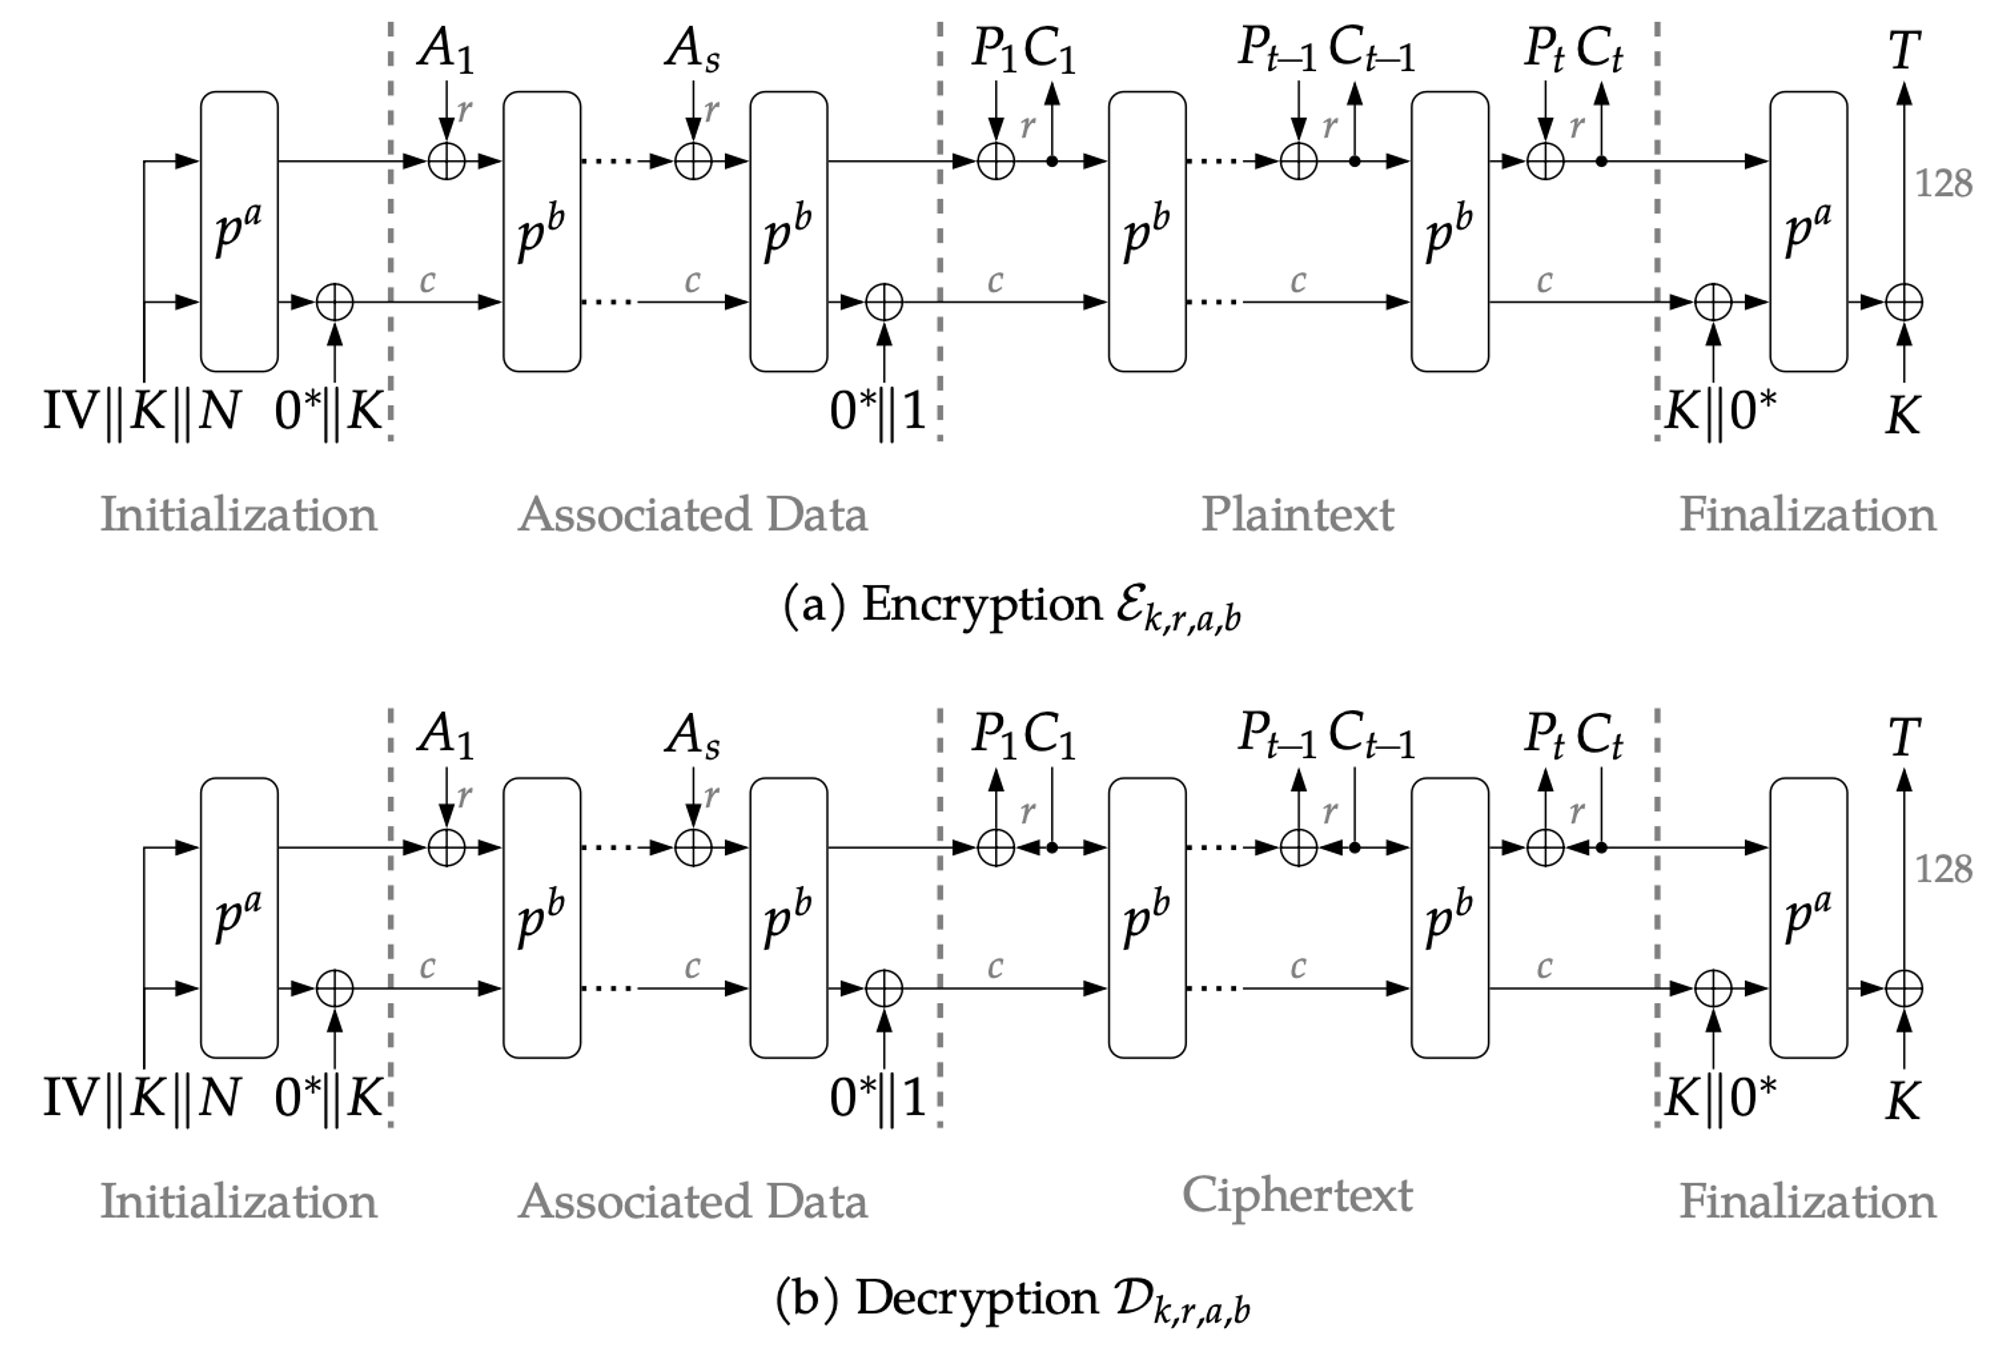
\includegraphics[width=1\textwidth]{figures/aead-algorithm.png}
    \caption{Ascon's mode of operation \cite{Ascon-v1.2}}
    \label{fig:aead-algorithm}
\end{figure}
\subsubsection{Initialization}
"The 320-bit initial state of Ascon is formed by [concatenating] the secret key K of k bits and nonce N of 128 bits, as well as an IV specifying the algorithm (including the key size k, the rate r, the initialization and finalization round number a, and the intermediate round number b, each written as an 8-bit integer)", followed by padding of 0s for the required length. 
$$S \leftarrow k || r || a || b || 0^{160-k} || K || N $$
In the Initialization $a$ rounds of the permutation $p$ is applied to the initial state. After that, the resulting state is XORed with a modified version of the secret key $K$ which is prepended with a series of $320-k$ zeros to pad it to the size of 320 bits. \cite{Ascon-v1.2}
$$S \leftarrow p^a(S) \oplus (0^{320-k} || K)$$
This step is needed to... 
\subsubsection{Processing Associated Data}
If there is associated data, it will first be preprocessed for absorbtion into blocks of $r$ bits which will be appended by a single $1$ and the smallest number of zeros to obtain a multiple of $r$ and then split again in $s$ blocks of $r$ bits. If there is no associated data, no padding is apllied and $s=0$.
The associated data $A$ is then absorbed into the state.
$$ S \leftarrow p^b((S_r \oplus A_i) || S_c),\ \ 1 \leq i \leq s$$
After all associated data is absorbed, a domain separation constant is added to differentiate the processing of associated data from the encryption of the payload. 
% which attacks?
This helps in avoiding certain types of cryptographic attacks. \dots
$$S \leftarrow S \oplus (0^{319} || 1)$$
\cite{Ascon-v1.2}
\subsubsection{Processing Plaintext/Ciphertext}
As for the payload it is also processed into blocks the same way. 
$$P_1, \dots , P_t \leftarrow \ r-bit blocks of P || 1 || 0^{r-1-(|P| mod\ r)}$$
For encryption each padded plaintext block $P_i$ is XORed to the first $r$ bits $S_r$ of the state $S$ and for each block except the last one is it is transformed by the permutation $p^b$% why???
$$C_i \leftarrow S_r \oplus P_i$$
% fix this
% $$
% s \leftarrow \begin{cases} 
%     p^b(C_i \parallel S_c) & \text{if } 1 \leq i < t \\
%     C_i \mid S_c & \text{if } i = t
%     \end{cases}
% $$
The last remaining block $C_t$ the padding is removed. This ensures that the decrypted plaintext matches the original plaintext exactly, without any additional padding bytes affecting the integrity of the data.
% $$\tilde{C}_t \leftarrow \left| C_t \right|_{|P|\ mod\ r}$$ % fix this to be truncated
\newline
To decrypt the ciphertext back the its original, each ciphertextblock except the last one is being XORed with the first $r$ bits $S_r$ of the internal state, which then has to be replaced by $C_i$ and then transformed by the $b$-round permutation $p^b$:
$$ P_i\leftarrow S_r \oplus C_i $$
$$ S \leftarrow (S_r \oplus (\tilde P_t || 1 || 0^{r-1-l})) || S_c $$
For the remaining truncated ciphertextblock $\tilde C_t\ with\ 0 \leq l \le r$ bits, the procedure differs:
$$\tilde{P}_t \leftarrow \left| S_r \right|_\ell \oplus \tilde{C}_t$$
$$S \leftarrow (S_r \oplus (\tilde P_t || 1 || 0^{r-1-l})) || S_c$$
\cite{Ascon-v1.2}
\subsubsection{Finalization}
\subsection{Procedures}